\chapter{Berechenbarkeitstheorie}
\section{Berechenbarkeiten}
\begin{center}
	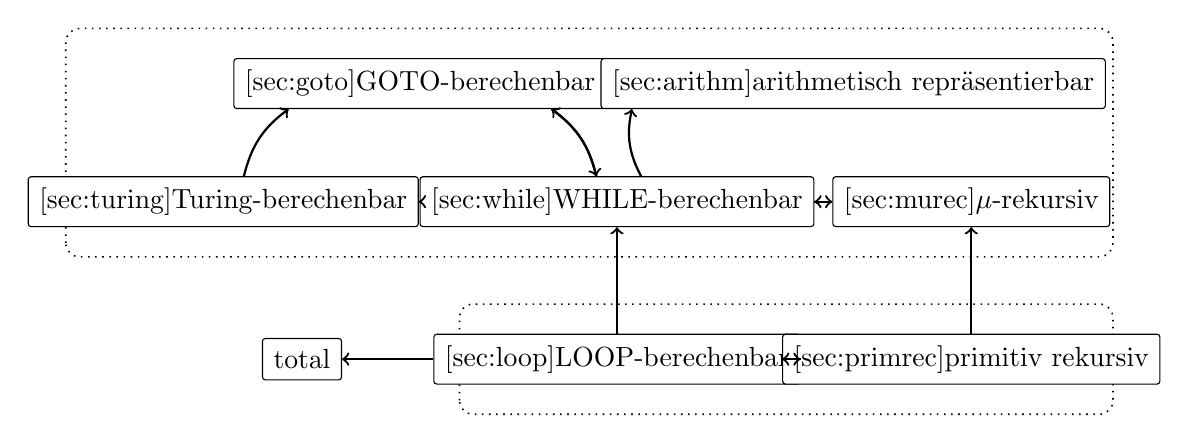
\begin{tikzpicture}
		\tikzset{
			grouplabel/.style={
				draw,
				fill = white,
				rectangle,
				inner sep = 4pt,
				rounded corners=1pt
			}
		}

		\draw [rounded corners=5pt, dotted, line width=0.2mm] (0,6.3) rectangle (13.3,9.2);
		\draw node (tm) at (2,7) [grouplabel] {\hyperref[sec:turing]{Turing-berechenbar}};
		\draw node (while) at (7,7) [grouplabel] {\hyperref[sec:while]{WHILE-berechenbar}};
		\draw node (goto) at (4.5,8.5) [grouplabel] {\hyperref[sec:goto]{GOTO-berechenbar}};
		\draw node (mu) at (11.5,7) [grouplabel] {\hyperref[sec:murec]{$\mu$-rekursiv}};
		\draw node (arm) at (10,8.5) [grouplabel] {\hyperref[sec:arithm]{arithmetisch repräsentierbar}};

		\draw [rounded corners=5pt, dotted, line width=0.2mm] (5,4.3) rectangle (13.3,5.7);
		\draw node (loop) at (7,5) [grouplabel] {\hyperref[sec:loop]{LOOP-berechenbar}};
		\draw node (prek) at (11.5,5) [grouplabel] {\hyperref[sec:primrec]{primitiv rekursiv}};
		\draw node (total) at (3,5) [grouplabel] {total};

		\draw[thick, ->] (while) to (tm);
		\draw[thick, ->] (tm) to[bend left=20] (goto);
		\draw[thick, ->] (goto) to[bend left=20] (while);
		\draw[thick, ->] (while) to[bend right=20] (goto);
		\draw[thick, ->] (mu) to (while);
		\draw[thick, ->] (while) to (mu);
		\draw[thick, ->] (while) to[bend left=20] (arm);

		\draw[thick, ->] (prek) to (mu);
		\draw[thick, ->] (loop) to (while);
		\draw[thick, ->] (loop) to (prek);
		\draw[thick, ->] (prek) to (loop);

		\draw[thick, ->] (loop) to (total);
	\end{tikzpicture}
\end{center}

\vspace{2em}
Einige Funktionen, in den einzelnen Berechenbarkeitsklassen
\vspace{1em}

\begin{center}
	\begin{tikzpicture}
		\tikzset{
			grouplabel/.style={
				draw,
				fill = white,
				rectangle,
				inner sep = 4pt,
				rounded corners=1pt
			}
		}

		\draw [rounded corners=5pt, dotted, line width=0.2mm] (0,0) rectangle (13.3,6.5);
		\draw [rounded corners=5pt, dotted, line width=0.2mm, fill=white] (-0.2,6) rectangle (13.5,11);

		\draw node (tm) at (7,11) [grouplabel] {WHILE/GOTO/Turing-berechenbar \& $\mu$-rekursiv};
		\draw node (while) at (7,6) [grouplabel] {LOOP-berechenbar \& primitiv rekursiv};


		\draw node[text width=12.5cm, align=left, anchor=north west] at (-0.2,10.5) {
		\parbox{\textwidth}{
		\begin{itemize}
			\item Ackermannfunktion
			\item
		\end{itemize}
		}};


		\draw node[text width=12.5cm, align=left, anchor=north west] at (0,6) {
		\parbox{\textwidth}{
		\begin{itemize}
			\item Cantor'sche Paarungsfunktion $c(x,y)=\binom{x+y+1}{2}+x$
			mit den Umkehrungsfunktionen $e(c(x,y))=x$ und $f(c(x,y))=y$.
			\item Beschränkter $\mathrm{max}$-Operator bzw. der beschränkte Existenz-Operator
		\end{itemize}
		}};
	\end{tikzpicture}
\end{center}




\subsection{LOOP-Berechenbarkeit}\label{sec:loop}
Eine Funktion $f:\N^k\rightarrow \N$ heißt LOOP-berechenbar,  falls es ein LOOP-Program $P$ gibt, das gestartet auf der Eingabe $n_1,n_2,\ldots,n_k$ in den Variablen $x_1,x_2,\ldots,x_n$ nach endlich vielen Schritten hält und die Variable $x_0$ den Wert $f(n_1,\ldots,n_k)$ beinhaltet.
\subsubsection{Erlaubte Basisanweisungen}
\begin{itemize}
	\item $x_i\coloneqq x_j+c$ bzw. $x_i\coloneqq x_j-c$ mit $c\in\N$
	\item \texttt{LOOP} $x_i$ \texttt{DO} $P$ \texttt{END}
	\item Hintereinanderausführung von LOOP-Programmen
\end{itemize}
\subsubsection{Simulierbare Makros}
\begin{itemize}
	\item Wertzuweisungen $x_i\coloneqq x_j$ und $x_i\coloneqq c$
	\item \texttt{IF} $x_i>c$ \texttt{THEN} $P$ \texttt{END}
	\item Alle üblichen arithmetischen Operationen, auch Modulrechnung
\end{itemize}

\subsection{WHILE-Berechenbarkeit}\label{sec:while}
Eine Funktion $f:\N^k\rightarrow \N$ heißt WHILE-berechenbar,  falls es ein WHILE-Program $P$ gibt, das gestartet auf der Eingabe $n_1,n_2,\ldots,n_k$ in den Variablen $x_1,x_2,\ldots,x_n$ nach endlich vielen Schritten hält (falls das Ergebnis definiert ist) und die Variable $x_0$ den Wert $f(n_1,\ldots,n_k)$ beinhaltet. Ist $f(n_1,\ldots,n_k)$ undefiniert, so hält $P$ nicht.

\begin{enumerate}
	\item Jedes GOTO-Programm kann durch ein WHILE-Programm mit nur einer einzigen WHILE-Schleife simuliert werden.
	\item Jede WHILE-Berechenbare Funktion kann durch ein WHILE-Programm mit nur einer einzigen WHILE-Schleife berechnet werden (Kleene'sches Normalform-Theorem)
\end{enumerate}

\subsubsection{Erlaubte Anweisungen}
\begin{itemize}
	\item Alle Anweisungen von LOOP-Programmen
	\item \texttt{WHILE} $x_i\neq 0$ \texttt{DO} $P$ \texttt{END}
\end{itemize}


\subsection{GOTO-Berechenbarkeit}\label{sec:goto}
\subsubsection{Erlaubte Anweisungen}
\begin{itemize}
	\item Berechnungen und Zuweisungen: $x_i\coloneqq x_j\pm c$
	\item Marken: $M_i$
	\item \texttt{GOTO} $M_i$
	\item \texttt{HALT}
	\item \texttt{IF} $x_i=c$ \texttt{THEN GOTO} $M_j$
\end{itemize}
\subsubsection{Simulierbare Makros}
\begin{itemize}
	\item Die \texttt{WHILE}-Schleife
\end{itemize}

\subsection{Turing-Berechenbarkeit}\label{sec:turing}
Eine Funktion $f:\N^k\rightarrow \N$ heißt Turing-berechenbar, falls eine deterministische Turingmaschine existiert, die $f(n_1,\ldots,n_k)=m$ berechnet indem, sie gestartet auf dem $k$-Tupel $(n_1,\ldots,n_k)$ nach endlich vielen Berechnungsschritten einen Endzustand erreicht und dann $m$ auf dem Band steht. Falls das Ergebnis für die Eingabe undefiniert ist, terminiert die Maschine nie.

\subsection{Primitive Rekursion}\label{sec:primrec}
Eine Funktion ist genau dann primitiv rekursiv, wenn sie LOOP-berechenbar ist.
\begin{itemize}
	\item Konstante Funktionen sind primitiv rekursiv
	\item Projektionen sind primitiv rekursiv
	\item Die Nachfolgerfunktion $s:\N\rightarrow\N, n\mapsto n+1$ ist primitiv rekursiv
	\item Verkettungen von primitiv rekursiven Funktionen sind primitiv rekursiv
	\item Funktionen, die durch primitive Rekursion aus primitiv rekursiven Funktionen entstehen, sind primitiv rekursiv:
	\begin{align*}
		f(0,x_1,\ldots,x_k)&=g(x_1,\ldots,x_k) &&\text{(Startwert)}\\
		f(n+1,x_1,\ldots,x_k)&=h(f(n,x_1,\ldots,x_k),n,x_1,\ldots,x_k) &&\text{(Rekursionsschritt)}
	\end{align*}
	Das heißt, $g, h$ primitiv rekursiv $\Rightarrow$ $f$ primitiv rekursiv.
\end{itemize}

\subsection{$\mu$-Rekursion}\label{sec:murec}
\begin{equation*}
	\mu f(x_1,\ldots,x_k)=\min \set{n\in\N}{f(n,x_1,\ldots,x_k)=0 \wedge \forall m<n:f(m,x_1,\ldots,x_k)>0}
\end{equation*}
Der $\mu$-Operator liefert den kleinsten Eingabewert $n$ der ersten Variable, bei der die Funktion $0$ ausgibt. Dabei muss insbesondere $f$ für alle Werte kleiner als $n$ definiert sein, da sonst eine Berechnung nicht möglich wäre.

\paragraph{Satz von Kleene:} Eine $\mu$-rekursive Funktion $f:\N^n\rightarrow\N$ lässt sich immer durch zwei $n+1$-stellige primitiv rekursive Funktionen darstellen:
\begin{equation*}
	f(x_1,\ldots,x_n)=p(x_1,\ldots,x_n,\mu q(x_1,\ldots,x_n))
\end{equation*}

\subsection{Arithmetische Repräsentierbarkeit}\label{sec:arithm}
Eine Funktion $f:\N^k\rightarrow \N$ heißt arithmetisch repräsentierbar, falls es eine $(k+1)$ stellige arithmetische Formel $F$ gibt, so dass gilt
\begin{equation*}
	F(n_1,\ldots,n_k,m)\Leftrightarrow f(n_1,\ldots,n_k)=m
\end{equation*}
Hierfür besteht eine arithmetische Formel zunächst aus Termen:
\begin{itemize}
	\item Alle $n\in\N$ sind Terme
	\item Für alle $i\in\N$ ist $x_i$ ein Term
	\item Verknüpfung zweier Terme mit $+$ oder $\ast$ sind ebenfalls Terme
\end{itemize}
Aus den Termen werden Formeln gebildet
\begin{itemize}
	\item Gleichheit zweier Terme $(t_1=t_2)$ ist eine Formel
	\item Für $F,G$ Formeln sind auch $\neg F, (F\wedge G)$ und $(F\vee G)$ Formeln
	\item Für $F$ eine Formel und $i\in\N$ sind auch $\forall x_i F$ und $\exists x_i F$ Formeln
\end{itemize}

\paragraph{Gödel'scher Unvollständigkeitssatz}
Jedes Beweissystem, das nur wahre Formeln der Arithmetik beweist muss unvollständig sein.
